\chapter{Principes théoriques de base}
\label{chap:principes-theoriques}

\section{Définitions}

Voici quelques définitions nécessaires à la bonne compréhension du rapport de travail de bachelor :

\begin{itemize}
    \item \textbf{Réserve de marche} : durée pendant laquelle un mouvement de montre, une fois entièrement remonté (ou chargé), 
    est capable de fournir le couple nécessaire à son fonctionnement sans être remonté que se soit manuellement ou par le mouvement d'une masse oscillante. 
    Il s’agit donc du temps pendant lequel la montre continue de fonctionner avant de s’arrêter.

    \item \textbf{Barillet} : organe du mouvement horloger qui contient le ressort moteur. 
    Il sert à stocker l’énergie mécanique lors du remontage de la montre et à la restituer progressivement au train de rouages pour assurer le fonctionnement du mouvement pendant la durée de la réserve de marche. 
    Le barillet est généralement constitué d’un tambour cylindrique, de son couvercle et de son arbre.

    \item \textbf{Cliquet d'armage} : mécanisme anti-retour associé au système de remontage. 
    Il permet de transmettre l’effort de remontage au barillet tout en empêchant celui-ci de se détendre en sens inverse. 
    Le cliquet d’armage agit comme un dispositif de verrouillage unidirectionnel, garantissant que l’énergie accumulée dans le ressort moteur ne se libère que par le train de rouages.
\end{itemize}

\section{Fonctionnement d'un mouvement de montre} 

Une montre mécanique est une montre qui n'utilise pas de pile pour fonctionner. Par conséquent,l'énergie nécesaire au bon fonctionnement du mouvement provient d'un système complexe qui convertit l'énergie stockée dans un ressort.

Au cœur du mouvement, se trouve le barillet, un ressort hélicoïdal enroulé sur lui-même, stockant l'énergie mécanique fournie lors du remontage de la montre grâce a une rotation de la couronne ou un mouvement de la masse oscillation. À mesure que le ressort se détend, il libère progressivement cette énergie à travers un système d'engrenages et de leviers, ce qui alimente les aiguilles de la montre. Ce ressort se détend sur une période de plusieurs heures.

Le couple fourni par le barillet varie en fonction du temps comme le montre le graphe : 

\begin{figure}[H]
  \centering
  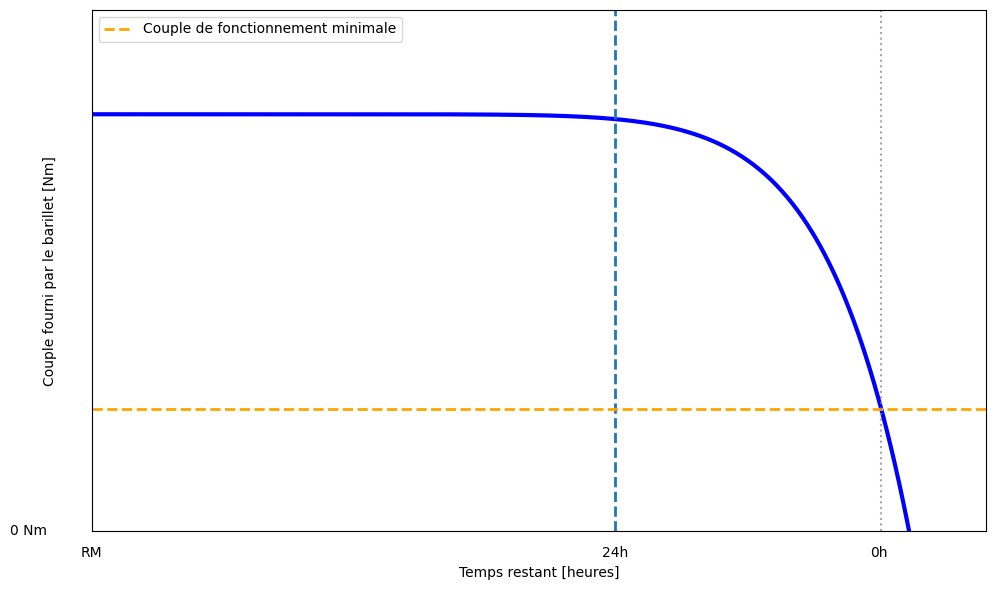
\includegraphics[width=1\textwidth]{assets/figures/Principes théoriques/graphe couple barillet.png}
  \caption{Évolution du couple fourni par le barillet en fonction du temps}
  \label{fig:couple_barillet}
\end{figure}

\section{Mesure accélérée de la réserve de marche par dévalement}

La technique de mesure accélérée utilisé lors de ce travail de Bachelor, consiste à enlever le cliquet d'armage du mouvement. Cette pièce a pour fonction de retenir le barillet et ainsi empêche le ressort du barillet de se dévaler en tournant librement. En prenant en considération que le ressort se déroule d'un nombre constant de tour par heure de fonctionnement de la montre et que le couple visible sur la figure \ref{fig:couple_barillet} est approximativement linéaire avant les 24 dernières heures de la réserve de marche. On peut établir une relation entre le nombre d'heures de réserve de marche et le nombre de tours de barillet durant cette phase linéaire, ce qui veut dire qu'en mesurant le temps d'un seul tour durant cette phase on peut ensuite regarder de combien de tour le barillet doit se dérouler et en déduire la réserve de marche complète du mouvement. 

Une fois cette durée calculé il reste à mesurer la phase non linéaire de manière classique.